
\subsection{RenderScript}
RenderScript is Android's official computing framework and was released in 
2011~\cite{RenderScript}. The motivation behind it is similar to that of OpenCL: to provide
performance and portability across SoC architectures for Android devices.
It accomplishes portability across devices by not exposing any architectural details to the programmer.

A RenderScript application consists of three parts: (1) Java application host
code written by the developer that runs on Dalvik VM, (2) RenderScript code
written in restricted C99 syntax containing one or more kernels, and (3)
auto-generated Java code that helps the application host code to communicate with
the RenderScript kernel code, allowing functions such as memory binding between the
host program and the kernels.

\begin{figure}
\centering
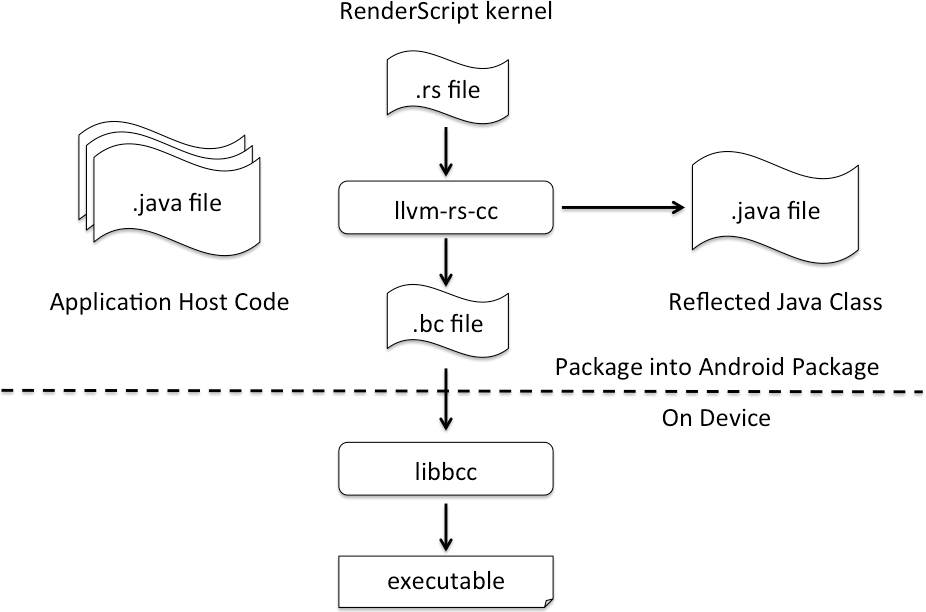
\includegraphics[scale=0.28]{figs/renderscript-compile.png}
\caption{RenderScript Compilation Flow}
\label{fig:RSCompilation}
\centering
\end{figure}

RenderScript compilation flow is shown in Figure~\ref{fig:RSCompilation}.
First, \fix{llvm-rs-cc} utility is used to compile RenderScript kernels to
LLVM~\cite{LLVM:CGO04} bitcode files. The LLVM IR provide support for a wide range of hardware
devices including CPUs, GPUs and DSPs. 
As part of the RenderScript compilation step, a Java class
is generated for each RenderScript file via the \fix{llvm-rs-cc} tool.
The generated Java classes essentially avoids the user having to write JNI code.
Then after, the application host code, the reflected Java classes, and RenderScript bitcode
are bundled together into the Android application package (\fix{*.apk} file).
During execution, the RenderScript
runtime invokes \fix{libbcc}, the RenderScript back-end compiler, to translate
bitcode into machine assembly.


